% Options for packages loaded elsewhere
\PassOptionsToPackage{unicode}{hyperref}
\PassOptionsToPackage{hyphens}{url}
\PassOptionsToPackage{dvipsnames,svgnames,x11names}{xcolor}
\documentclass[
  11pt,
]{article}
\usepackage{xcolor}
\usepackage[margin=1in]{geometry}
\usepackage{amsmath,amssymb}
\setcounter{secnumdepth}{-\maxdimen} % remove section numbering
\usepackage{iftex}
\ifPDFTeX
  \usepackage[T1]{fontenc}
  \usepackage[utf8]{inputenc}
  \usepackage{textcomp} % provide euro and other symbols
\else % if luatex or xetex
  \usepackage{unicode-math} % this also loads fontspec
  \defaultfontfeatures{Scale=MatchLowercase}
  \defaultfontfeatures[\rmfamily]{Ligatures=TeX,Scale=1}
\fi
\usepackage{lmodern}
\ifPDFTeX\else
  % xetex/luatex font selection
\fi
% Use upquote if available, for straight quotes in verbatim environments
\IfFileExists{upquote.sty}{\usepackage{upquote}}{}
\IfFileExists{microtype.sty}{% use microtype if available
  \usepackage[]{microtype}
  \UseMicrotypeSet[protrusion]{basicmath} % disable protrusion for tt fonts
}{}
\makeatletter
\@ifundefined{KOMAClassName}{% if non-KOMA class
  \IfFileExists{parskip.sty}{%
    \usepackage{parskip}
  }{% else
    \setlength{\parindent}{0pt}
    \setlength{\parskip}{6pt plus 2pt minus 1pt}}
}{% if KOMA class
  \KOMAoptions{parskip=half}}
\makeatother
\usepackage{longtable,booktabs,array}
\newcounter{none} % for unnumbered tables
\usepackage{calc} % for calculating minipage widths
% Correct order of tables after \paragraph or \subparagraph
\usepackage{etoolbox}
\makeatletter
\patchcmd\longtable{\par}{\if@noskipsec\mbox{}\fi\par}{}{}
\makeatother
% Allow footnotes in longtable head/foot
\IfFileExists{footnotehyper.sty}{\usepackage{footnotehyper}}{\usepackage{footnote}}
\makesavenoteenv{longtable}
\usepackage{graphicx}
\makeatletter
\newsavebox\pandoc@box
\newcommand*\pandocbounded[1]{% scales image to fit in text height/width
  \sbox\pandoc@box{#1}%
  \Gscale@div\@tempa{\textheight}{\dimexpr\ht\pandoc@box+\dp\pandoc@box\relax}%
  \Gscale@div\@tempb{\linewidth}{\wd\pandoc@box}%
  \ifdim\@tempb\p@<\@tempa\p@\let\@tempa\@tempb\fi% select the smaller of both
  \ifdim\@tempa\p@<\p@\scalebox{\@tempa}{\usebox\pandoc@box}%
  \else\usebox{\pandoc@box}%
  \fi%
}
% Set default figure placement to htbp
\def\fps@figure{htbp}
\makeatother
\setlength{\emergencystretch}{3em} % prevent overfull lines
\providecommand{\tightlist}{%
  \setlength{\itemsep}{0pt}\setlength{\parskip}{0pt}}
% Preamble injected into the pandoc LaTeX build (see scripts/build_paper.sh).
% Two jobs: (1) render inline Unicode math symbols correctly under XeTeX/tectonic
% by mapping each to its LaTeX math form; (2) keep wide tables from overflowing.

\usepackage{newunicodechar}
% --- math relations / operators ---
\newunicodechar{×}{\ensuremath{\times}}
\newunicodechar{·}{\ensuremath{\cdot}}
\newunicodechar{−}{\ensuremath{-}}
\newunicodechar{≤}{\ensuremath{\le}}
\newunicodechar{≥}{\ensuremath{\ge}}
\newunicodechar{≈}{\ensuremath{\approx}}
\newunicodechar{≫}{\ensuremath{\gg}}
\newunicodechar{∩}{\ensuremath{\cap}}
\newunicodechar{⋃}{\ensuremath{\bigcup}}
\newunicodechar{⊆}{\ensuremath{\subseteq}}
\newunicodechar{Σ}{\ensuremath{\Sigma}}
\newunicodechar{→}{\ensuremath{\rightarrow}}
% --- greek ---
\newunicodechar{φ}{\ensuremath{\varphi}}
\newunicodechar{ψ}{\ensuremath{\psi}}
\newunicodechar{ε}{\ensuremath{\varepsilon}}
\newunicodechar{µ}{\ensuremath{\mu}}
% --- sub/superscripts that appear inline ---
\newunicodechar{²}{\textsuperscript{2}}
\newunicodechar{ᵢ}{\textsubscript{i}}
\newunicodechar{ⱼ}{\textsubscript{j}}
\newunicodechar{₁}{\textsubscript{1}}
\newunicodechar{ₖ}{\textsubscript{k}}
\newunicodechar{ₘ}{\textsubscript{m}}

% --- diagrams ---
\usepackage{tikz}
\usetikzlibrary{positioning, arrows.meta, fit, backgrounds}

% --- keep wide tables inside the margins ---
\usepackage{etoolbox}
\AtBeginEnvironment{longtable}{\footnotesize}
\AtBeginEnvironment{tabular}{\small}
\setlength{\tabcolsep}{4pt}
\usepackage{bookmark}
\IfFileExists{xurl.sty}{\usepackage{xurl}}{} % add URL line breaks if available
\urlstyle{same}
% fallback for those not using the hyperref driver hyperxmp:
\makeatletter
\@ifundefined{xmpquote}{\newcommand{\xmpquote}[1]{#1}}{}
\makeatother
\hypersetup{
  pdftitle={Recovering Repeated Structure in Flat 2D Rectilinear Layouts: A Geometry-First Framework Unifying Array Detection and Hierarchy Recovery},
  colorlinks=true,
  linkcolor={blue},
  filecolor={Maroon},
  citecolor={Blue},
  urlcolor={blue},
  pdfcreator={LaTeX via pandoc}}

\title{Recovering Repeated Structure in Flat 2D Rectilinear Layouts: A
Geometry-First Framework Unifying Array Detection and Hierarchy
Recovery}
\author{}
\date{July 2026}

\begin{document}
\maketitle

{
\setcounter{tocdepth}{3}
\tableofcontents
}
\emph{Draft --- internal working version. All numbers are from measured
runs of the implemented C++/Boost.Geometry system (synthetic benchmarks
and a real \texttt{gdstk} GDS round-trip). The one remaining open item
--- running the identical harness on a real SKY130/ORFS \texttt{.gds}
crop --- is marked \texttt{{[}TBD{]}}.}

\begin{center}\rule{0.5\linewidth}{0.5pt}\end{center}

\section{1. Abstract}\label{abstract}

Flat 2D geometric layouts --- integrated-circuit masks after hierarchy
flattening, tiled facades, decorative patterns, printed arrays ---
routinely contain repeated structure that was present as
\emph{step-and-repeat} metadata upstream but is lost once the geometry
is reduced to a single flat pool of polygons. Recovering that structure
is valuable for compression, verification, and layout analysis, but it
is hard precisely because the repetition is usually \emph{partial}: a
regular region embedded in clutter, borders, routing, and localized
defects, rather than a globally periodic image.

We present a single geometry-first framework that recovers repeated
structure across the full spectrum from a rigid lattice \textbf{array}
to an arbitrary nested \textbf{hierarchy} of reusable cell definitions
and instance placements. The framework rests on two shared ideas. First,
\textbf{symbolic string / local-hash methods are candidate generators,
never proofs}: they are cheap, lossy filters that propose where
repetition might live; only \textbf{canonicalized geometric equality}
certifies it. Second, \textbf{a minimum-description-length (MDL)
objective} decides which repeated substructures are worth promoting to
cells. The central claim, and the organizing thesis of this paper, is
that \textbf{array detection is exactly the one-level, lattice-aligned
special case of hierarchy recovery} --- not merely analogous to it. We
demonstrate this empirically: on the same flattened layout, the
dedicated array detector and a one-level run of the hierarchy recoverer
followed by a lattice fit produce \textbf{identical lattice parameters}
(step vectors and grid) with equivalent total site accounting, differing
only in one modal-cell attribution on the standard-cell case (§7.2).

The framework is implemented in C++17 on Boost.Geometry. It reproduces
three previously-diagnosed bug classes as passing regression tests,
recovers both decorative and standard-cell demo layouts (including
directly-abutted zero-gap geometry that a single encoding cannot
handle), recovers D4-oriented (mirrored/rotated) instances as one cell,
and passes both a synthetic and a \textbf{real-GDS} hierarchy-erasure
benchmark with exact flatten-equality --- 3.3--3.5× compression on the
synthetic datapaths and 3.80× on the real-GDS round-trip --- recovering
the leaf cell in every case. (An earlier, higher compression figure came
from an over-covering verification bug; the corrected, exact-multiset
verification both fixed it and lowered the honest number ---
verification is a correctness gate, not just a metric.) Performance is
linear at roughly 3 µs per rectangle; 1.58 M rectangles recover in about
4.8 s single-round (about 30 s under full recursion) on one core. The
real-GDS evaluation writes and flattens a genuinely hierarchical layout
with \texttt{gdstk} and recovers from the flat rectangles.

Throughout we follow the design documents' insistence on honesty about
scope and claims: the recovered hierarchy is \emph{one} of many valid
decompositions of the same flat geometry, so where ground truth exists
we report \textbf{agreement, not accuracy}.

\begin{center}\rule{0.5\linewidth}{0.5pt}\end{center}

\section{2. Introduction}\label{introduction}

\subsection{2.1 Motivation}\label{motivation}

A modern integrated-circuit layout is authored hierarchically: a
designer defines a small cell (a logic gate, a bit-slice, an SRAM bit),
and place-and-route tools instantiate it thousands or millions of times,
often on regular rows and arrays with array-reference (AREF) metadata
recording the step and count compactly. This hierarchy is what keeps a
GDSII/OASIS file for a billion-transistor chip a manageable size. But
many downstream operations --- DRC region extraction, third-party IP
analysis, reverse engineering of a flattened block, mask-data-prep
tooling --- receive geometry that has already been \textbf{flattened}:
the cell and array references are expanded into raw polygons and the
hierarchy metadata is gone. The same happens in non-IC settings: a
decorative tiling, a rendered pattern, or a scanned facade arrives as
flat geometry with its generative structure implicit.

Recovering the lost structure directly from geometry has concrete
payoffs. If a region is a genuine array, reporting it as
\texttt{(tile,\ step-x,\ step-y,\ count)} plus a short defect list is
dramatically smaller than the expanded polygon set, and it exposes the
array's \emph{defects} (a missing instance, an extra overlaid polygon)
as first-class findings. More generally, inferring a compact hierarchy
re-compresses a flattened layout and can reveal design intent that the
flattening erased.

\subsection{2.2 The problem, and why it is not just ``find the
period''}\label{the-problem-and-why-it-is-not-just-find-the-period}

Two properties make this hard and distinguish it from classic
periodicity detection:

\begin{itemize}
\tightlist
\item
  \textbf{Partiality.} The layout is \emph{not} globally periodic. An
  array occupies a rectangular sub-region while borders, routing,
  filler, and unrelated blocks surround it. Multiple distinct arrays may
  coexist. A global-periodicity method (autocorrelation, global Fourier
  peak) answers the wrong question; it assumes the whole image repeats.
\item
  \textbf{Representation slack.} The same logical geometry can be
  represented by different polygon decompositions --- fractured versus
  merged, different winding, near-duplicate coordinates from
  floating-point noise. Any comparison that is naive about
  representation will reject valid repeats for non-geometric reasons.
\end{itemize}

The framework confronts both directly: repetition evidence is gathered
\emph{locally} (line-wise runs, local geometric neighborhoods) so
partiality is natural, and every acceptance decision routes through
\textbf{canonicalized} geometric comparison so representation slack is
neutralized.

\subsection{2.3 Contributions}\label{contributions}

\begin{itemize}
\tightlist
\item
  \textbf{A unified geometry-first framework} covering the whole range
  from rigid lattice arrays to arbitrary nested hierarchy, built on two
  shared mechanisms: canonicalized geometric verification as the sole
  certifier, and an MDL compression-gain objective as the promotion
  rule.
\item
  \textbf{An empirical demonstration of the unification}: array
  detection is realized as one-level hierarchy recovery plus a lattice
  fit, and the two paths produce identical lattice parameters
  (\texttt{dx}, \texttt{dy}, grid) with equivalent total site accounting
  --- differing only in one modal-cell attribution on the standard-cell
  case (§7.2). This makes ``array detection is a special case of
  hierarchy recovery'' a demonstrated equality rather than a framing
  convenience.
\item
  \textbf{Two complementary symbolic encodings} (occupancy-interval and
  edge-boundary) that together handle both gapped and directly-abutted
  (zero-gap) geometry --- a case a single encoding provably fails on.
\item
  \textbf{A period-phase reconciliation formulation} as clustering over
  physical period, modular phase, and spatial support (with a
  center-pruning step that defeats the transitive weak-link failure
  mode), replacing ad hoc ``try-shifts'' alignment.
\item
  \textbf{A defect model} (\texttt{missing\ =\ expected\ −\ observed},
  \texttt{extra\ =\ observed\ −\ expected}) computed with exact
  geometry, and correctly attributed to physical positions across
  defects --- reproducing and guarding against three
  previously-diagnosed bug classes as regression tests.
\item
  \textbf{D4 orientation support} (the 8 axis-preserving
  reflections/rotations), so mirrored standard-cell rows recover as one
  cell rather than eight spurious ones.
\item
  \textbf{A linear-time implementation} and the finding that the
  algorithm itself was never the scaling bottleneck --- the
  \texttt{flatten(H)\ =\ G} verification was --- with the fix that
  restores linearity (§7.4).
\item
  \textbf{An exact O(n) rectangle-multiset verification used as a
  correctness gate}, not merely a metric: it caught an over-covering
  recovery bug (nested instances silently overlapping, rectangles
  double-counted) that a weaker \texttt{G\ ⊆\ flatten} check had
  rubber-stamped, and forced the honest compression numbers down (§6,
  §7.3, §7.5).
\end{itemize}

\begin{center}\rule{0.5\linewidth}{0.5pt}\end{center}

\section{3. Related Work}\label{related-work}

We situate the framework against three families, briefly and honestly.

\textbf{Global-periodicity methods.} Autocorrelation, Fourier-peak, and
lattice-from-image techniques recover a single dominant period for an
image or point set. They are efficient and well-understood, but they
assume global periodicity. Our target is the opposite regime --- a
partial array embedded in a mostly non-repeating layout --- where a
global period either does not exist or is dominated by clutter. We use
periodicity only \emph{line-wise and locally}, as candidate evidence,
never as a global assumption.

\textbf{Pairwise geometric motif matching.} One can search directly for
repeated geometry by comparing polygon neighborhoods against each other.
This is expressive but tends toward quadratic cost in the number of
primitives if done naively, and it needs a canonicalization to be
robust. We keep the canonicalized geometric comparison (it is our
certifier) but avoid the quadratic candidate search: array candidates
come from line-wise runs (linear per line), and hierarchy candidates
come from local geometric \emph{shingles} gathered through a spatial
index (an rtree), so candidate generation never pays the all-pairs cost.

\textbf{String maximal-repetition / grammar induction.} Linear-time
\emph{runs} algorithms find maximal periodic substrings; suffix
structures and grammar-induction methods (Sequitur, Re-Pair) find
repeated (not necessarily contiguous) substrings and are natively
aligned with a compression objective. We borrow these as
\emph{serialization-channel} candidate generators, but with an explicit
tool distinction the design documents make {[}v4, HR{]}: periodic
\emph{runs} fit adjacent-on-a-lattice array instances, whereas
\emph{repeated substrings} fit cell instances scattered with unrelated
content between them. Crucially, a string match over serialized geometry
is lossy --- serialization order is itself a choice, and tolerance
binning can preserve a symbolic period while the physical lattice drifts
--- so the string stage is a filter and the geometry stage is the proof.

The distinguishing stance of this work is the combination:
\textbf{partial} structure in clutter, \textbf{sub-quadratic} candidate
generation via line-runs and local shingles, \textbf{canonicalized
geometric certification}, and an \textbf{MDL} objective that ties the
whole thing to description-length reduction --- with array detection
falling out as a special case rather than being treated as a separate
problem.

\begin{center}\rule{0.5\linewidth}{0.5pt}\end{center}

\section{4. Problem Statement}\label{problem-statement}

\subsection{4.1 Array detection}\label{array-detection}

\textbf{Input.} A collection of axis-aligned rectangles in the plane
(the rectilinear scope means a rectangle is the only primitive we need;
a fractured polygon is several rectangles).

\textbf{Target.} A candidate array is a tuple \textbf{A = (B, u, v, T)}
where \texttt{B} is a rectangular bounding box, \texttt{u\ =\ (dx,\ 0)}
and \texttt{v\ =\ (0,\ dy)} are orthogonal lattice vectors, and
\texttt{T} is the tile geometry of one fundamental cell. The
\textbf{exact array condition} {[}v4, §1.2{]} is

\[G \cap B \;=\; \bigcup_{i,j} \big( (T + i\,\mathbf{u} + j\,\mathbf{v}) \cap B \big)
\qquad\text{(after coordinate snapping and canonicalization)}\]

The canonicalization qualifier is load-bearing: comparing raw, unsnapped
geometry would reject valid arrays for representational reasons. The
detector seeks a \textbf{primitive} tile (the smallest verified
repeating unit) but may report a \textbf{supercell} when primitive
recovery is ambiguous; a coincidental match that survives no candidate
period is a \textbf{pseudo-array} and is discarded {[}v4, §2.4{]}.

Importantly, the symbolic stage never establishes the exact array
condition directly. It establishes only a weaker \emph{necessary}
condition --- that many horizontal slabs are periodic in \texttt{x} with
period \texttt{dx}, and many vertical slabs periodic in \texttt{y} with
period \texttt{dy} --- which geometric verification then upgrades to the
full sufficient condition.

\subsection{4.2 Hierarchy recovery}\label{hierarchy-recovery}

\textbf{Input.} Flat polygon geometry \texttt{G} (again, rectangles
under our scope).

\textbf{Output.} A hierarchy \(H = (C_1..C_m,\ I_1..I_k,\ R)\) of cell
definitions, instance placements, and residual geometry, such that

\[\mathrm{flatten}(H) = G \quad\text{within tolerance } \varepsilon\]

minimizing

\[\mathrm{cost}(H) = \sum_i \mathrm{cost}\big(\mathrm{body}(C_i)\big) + \sum_j \mathrm{cost}\big(\mathrm{inst}(I_j)\big) + \mathrm{cost}\big(\mathrm{residual}(R)\big)\]

Cells may reference smaller cells (nested hierarchy), which is how
``arrays inside arrays'' are represented {[}HR, §1.1{]}. Candidate
generation is heuristic; only \texttt{flatten(H)\ =\ G}, checked by
canonicalized equality, certifies a hierarchy.

\subsection{4.3 Assumptions and scope}\label{assumptions-and-scope}

Shared by both problems {[}v4, §1.1; HR, §1.2{]}:

\begin{itemize}
\tightlist
\item
  \textbf{Axis-aligned, rectilinear (Manhattan)} geometry with an
  orthogonal two-vector lattice --- not arbitrary oblique lattices.
\item
  \textbf{Single-layer} geometry (multi-layer/multi-class is future
  work).
\item
  \textbf{Fractured polygons} are expected; verification must tolerate
  one logical shape represented as several rectangles.
\item
  \textbf{Exact repetition} (within tolerance ε) is the primary target;
  bounded-defect matching is a defined extension, not the default.
\item
  Holes and overlapping polygons are out of scope for the initial
  version.
\item
  \textbf{Transform scope.} Translation-only by default, deliberately
  \textbf{extended to the dihedral group D4} --- the 8 axis-preserving
  orientations (rotations by 0/90/180/270°, each optionally mirrored)
  --- because place-and-route flows routinely mirror alternating
  standard-cell rows to share a power rail. Under translation-only
  canonicalization a mirrored instance would register as unrelated
  geometry; instance records therefore carry an \textbf{orientation
  field}, not just a position {[}HR, §1.2{]}.
\end{itemize}

\subsection{4.4 Non-uniqueness (stated up
front)}\label{non-uniqueness-stated-up-front}

A flat layout generally admits \textbf{many} valid hierarchical
decompositions. \texttt{ABABABAB} flattens identically whether the
source was one cell \texttt{AB} × 4, alternating \texttt{A}/\texttt{B},
or \texttt{ABAB} × 2. The target is therefore \emph{a compact,
geometrically valid hierarchy}, not \emph{the designer's original
hierarchy}. Where evaluation compares against a known source, we report
\textbf{agreement}, not \textbf{accuracy} {[}HR, §1.3{]}. This is not a
caveat bolted on at the end; it shapes the evaluation (§7) and the
honest limitations (§8).

\begin{center}\rule{0.5\linewidth}{0.5pt}\end{center}

\section{5. Method}\label{method}

The pipeline maps 1:1 onto the design documents' sections and the
implemented C++ modules. Array detection runs stages 5.1--5.4; hierarchy
recovery reuses 5.1's snapping and 5.4's canonicalized-equality
machinery and adds 5.5--5.6.

\subsection{5.1 Scanline construction (coordinate snapping + open-slab
sampling)}\label{scanline-construction-coordinate-snapping-open-slab-sampling}

Scanlines are derived from the arrangement induced by rectangle
vertices, with two precision rules that matter for correctness {[}v4,
§2.1{]}:

\begin{itemize}
\tightlist
\item
  \textbf{Coordinate snapping before slab construction.} Raw coordinates
  are snapped to a tolerance grid (default 0.05) and coalesced, so
  near-duplicate coordinates do not fragment the layout into a blizzard
  of near-zero-height slabs. \texttt{X}, \texttt{Y} = unique snapped x-,
  y-coordinates.
\item
  \textbf{Open-slab sampling.} Consecutive \texttt{Y} values define open
  horizontal slabs; each non-empty slab is represented by a sample line
  strictly \emph{inside} the open interval (the midpoint), never on a
  boundary. For rectilinear polygons the intersection topology is
  constant for any horizontal line strictly inside one open slab, so one
  representative line fully characterizes it. Horizontal edges lie on
  slab boundaries and are represented through the boundary coordinates
  directly.
\end{itemize}

Vertical slabs are built symmetrically by treating \texttt{x} as the
scan-normal axis, so one code path
(\texttt{build\_slabs(axis\_swapped)}) serves both passes. Each slab
keeps two views: the \textbf{merged} covered intervals (for the
occupancy encoding) and the \textbf{raw per-rectangle spans} with their
heights (for the edge encoding, which must see internal boundaries the
merge would dissolve). Snapping and open-interval sampling compose:
snapping bounds the slab count, open sampling keeps each surviving slab
unambiguous; neither alone suffices.

\subsection{5.2 Two symbolic encodings}\label{two-symbolic-encodings}

Each slab is turned into a metric-preserving token stream --- every
token carries both a symbol and a physical length, because tolerance
binning is not automatically metric-preserving and reconciliation must
operate on the physical fields {[}v4, §2.2{]}.

\begin{itemize}
\tightlist
\item
  \textbf{Occupancy-interval encoding.} From the \emph{merged} covered
  intervals: filled tokens carry the quantized covered width, gap tokens
  the quantized empty width. Strong when features have real gaps between
  them.
\item
  \textbf{Edge-boundary encoding.} From the \emph{raw, unmerged}
  per-rectangle spans, each filled token keyed on
  \texttt{(width,\ edge-height)}, with no gap token between abutted
  cells. This is the concrete realization of ``every edge characterized
  by its projection vector'' specialized to axis-aligned boxes {[}NOTES,
  decision 9{]}.
\end{itemize}

\textbf{Why two encodings --- the zero-gap case.} Occupancy leans on gap
structure. Two directly-abutted cells with zero gap merge into one wide
covered interval, so occupancy cannot see the repeated boundary between
them; the edge encoding keeps them as two distinct tokens and recovers
the array. This is not hypothetical: the prototype implemented only
occupancy and its standard-cell demo had to insert artificial gaps to
work at all --- a live demonstration that one encoding is insufficient.
The C++ system implements both and recovers a genuinely zero-gap abutted
standard-cell array through the edge encoding (§7.1). Both filled tokens
get positive interned symbol ids and gap tokens negative, so downstream
code reads ``filled vs.~empty'' from the sign.

\subsection{5.3 Per-line repetition and period-phase
reconciliation}\label{per-line-repetition-and-period-phase-reconciliation}

\textbf{Per-line repetition} (\texttt{analyze\_row}) finds each slab's
primitive physical period. The implementation uses the prototype's O(n²)
self-consistency scan rather than a linear-time runs algorithm; both the
design and the prototype note this stage is swappable without downstream
impact {[}NOTES, decision 10{]}. The period chosen is the smallest one
whose majority-vote canonical unit actually \textbf{reproduces} the row
above a strict self-consistency floor --- \emph{not} merely the smallest
that clears a loose match fraction. This is exactly what defeats bug 2
(below): a half-period that matches only because two of four widths
coincide scores below the strict floor and loses to the true primitive.
The loose floor survives only to flag a genuine supercell (content
near-repeats at \texttt{d} but is truly invariant only at \texttt{k·d}).

Each run is recorded with both symbolic and physical fields, and its
phase is \texttt{φ\ =\ x\_start\ mod\ dx} using modular distance
\texttt{dist\_mod(a,b;p)\ =\ min(\textbar{}a−b\textbar{},\ p−\textbar{}a−b\textbar{})}.

\textbf{Reconciliation} (\texttt{cluster\_runs},
\texttt{intersect\_passes}) lifts the design's key correction into code:
rows within a tile need \emph{not} have identical content --- a row
crossing the top of a rectangle legitimately differs from one crossing
its middle. What must agree is each row's own internal periodicity,
matched on \textbf{physical step and phase}, not on symbol content
{[}v4, §2.4{]}. Two runs are compatible when

\[\begin{aligned}
|dx_i - dx_j| &\le \varepsilon_{\text{period}}, \\
\mathrm{dist\_mod}(\varphi_i, \varphi_j;\, dx) &\le \varepsilon_{\text{phase}}, \\
\mathrm{overlap}\big([x_{\text{start}}, x_{\text{end}}]_i,\, [\cdot]_j\big) &\ge w_{\min}.
\end{aligned}\]

Runs are clustered by \textbf{connected components} under this hard
pairwise predicate (the graph view of the design's clustering/voting
duality). To defeat the transitive weak-link problem the design warns
about (A\textasciitilde B and B\textasciitilde C compatible does not
make A\textasciitilde C good evidence), a robust cluster center is
computed --- \textbf{median} period and \textbf{circular-median} phase
--- and any member incompatible with that center is pruned, recomputing
once {[}NOTES, decision 2{]}. The circular median has no closed form
(phase wraps modulo the period); it is computed as the φ minimizing
\texttt{Σ\ dist\_mod(φ,\ φᵢ;\ p)} searched over the observed phases plus
pairwise midpoints and their antipodes {[}NOTES, decision 3{]}.

The same construction runs on \textbf{vertical} slabs, producing
\texttt{(dy,\ ψ)} votes. A 2D hypothesis is formed where a
horizontally-supported cluster and a vertically-supported cluster
overlap spatially and induce a consistent rectangle --- the horizontal ×
vertical intersection that yields the true 2D lattice. The candidate
rectangle is the \textbf{union} of member supports (the intersection
would collapse the rectangle to a single row whenever member supports
vary; since the compatibility predicate already requires pairwise
overlap, members are genuine co-lattice evidence and the union is the
honest footprint) {[}NOTES, decision 4{]}. Clusters are classified
primitive / supercell / pseudo-array; LCM combines periods only for runs
already classified as genuine-supercell evidence, never as a default
rule.

Pseudo-code for the reconciliation core:

\begin{verbatim}
function reconcile(row_runs):
    lines = [ project(r) for r in row_runs ]         # onto (scan, normal) axes
    graph = edges { (i,j) : compatible(lines[i], lines[j]) }
    for comp in connected_components(graph):
        p_star   = median(period over comp)
        phi_star = circular_median(phase over comp; period = p_star)
        comp = { r in comp : |period(r)-p_star| <= eps_p
                             and dist_mod(phase(r),phi_star;p_star) <= eps_phi }
        if |comp| >= min_members:
            emit cluster(period=p_star, phase=phi_star,
                         support=union(scan/normal extents))
    # symmetric vertical pass, then:
    return intersect(horizontal_clusters, vertical_clusters)
\end{verbatim}

\subsection{5.4 Geometric verification and defect
model}\label{geometric-verification-and-defect-model}

Reconciliation establishes only the necessary line-wise condition;
verification (\texttt{verify\_candidate}) upgrades a 2D hypothesis to a
certified array by canonicalized geometric comparison against the source
layout {[}v4, §2.5{]}:

\begin{enumerate}
\def\labelenumi{\arabic{enumi}.}
\tightlist
\item
  Clip the original geometry to the candidate rectangle.
\item
  Take the canonical tile as the \textbf{modal} cell content across all
  instances (not cell (0,0) blindly --- so one defective reference cell
  cannot define the tile everyone is measured against).
\item
  Translate tile copies across \texttt{(dx,\ dy)} to reconstruct the
  rectangle.
\item
  Canonicalize both (snap, normalize winding, merge coincident edges,
  sort rings) and compare. Only matching hypotheses are accepted.
\end{enumerate}

Because it is already clipping every expected instance, the same pass
computes the \textbf{§6 defect map} with Boost boolean ops:

\[\begin{aligned}
\text{missing} &= \text{expected} - \text{observed} && \text{(instance geometry incomplete — a structural defect)}\\
\text{extra} &= \text{observed} - \text{expected} && \text{(routing/clutter over a complete instance)}
\end{aligned}\]

An instance is \textbf{clean when none of its own geometry is missing};
overlaid extra geometry is reported separately (\texttt{n\_extra})
rather than making the instance a defect {[}NOTES, decision 6{]}. This
is what lets the standard-cell demo certify the array \emph{and} report
its routing overlays and its one genuine missing cell distinctly.
Critically --- and this is the concrete fix for bug 3 --- the defect
scan walks \textbf{expected physical positions}
\texttt{x\_start\ +\ m·dx}, looking up each position's actual geometry
by physical x-window, never by token index. A missing instance is
reported at its true \texttt{x}, and nothing after it desyncs {[}v4, §6;
NOTES, decision 5{]}.

\subsection{5.5 Hierarchy recovery}\label{hierarchy-recovery-1}

Hierarchy recovery (\texttt{recover\_hierarchy}) reuses 5.1's snapping
and 5.4's canonicalized equality, and adds candidate generation, MDL
scoring, selection, and recursion {[}HR, §2{]}.

\textbf{Channel B --- geometric shingles / local hashing.} Independent
of any global serialization, a small local neighborhood (a seed
rectangle plus its \texttt{k} nearest neighbors, \texttt{k\ =\ 1} by
default) is gathered around each rectangle through an rtree,
canonicalized to a translation- and D4-invariant signature, and hashed.
Neighborhoods that hash identically across locations are candidate
motifs. The seed is deliberately small: a large fixed neighborhood would
fold per-instance clutter into the signature and split true instances
apart {[}NOTES, Phase-2 decision 3{]}. The design designates Channel B
the primary, structurally sound generator because its recall does not
depend on a global traversal order; the multi-serialization Channel A is
a cheap but structurally incomplete supplement and is left unimplemented
pending an ablation {[}HR, §2.3; NOTES, Phase-2 decision 2{]}.

\textbf{Seed-and-extend growth.} Each small seed is grown geometrically:
for each occurrence, add a neighboring primitive only if it is present
at a \textbf{consistent offset around every occurrence simultaneously}.
Growth stops when no further addition holds across all instances, and is
rtree-local and size-capped (\texttt{max\_cell\_members}) so a perfectly
periodic region cannot grow an unbounded body. Because clutter is not
present at a consistent offset around every instance, it cannot attach
--- this is what keeps clutter out of cell bodies {[}HR, §2.4{]}.

\textbf{MDL compression gain.} For a candidate body \texttt{M} occurring
\texttt{k} times,

\[\mathrm{gain}(M) = (k-1)\cdot|\mathrm{body}(M)| \;-\; k\cdot\mathrm{cost\_instance} \;-\; \mathrm{def\_overhead}\]

The instance term scales with \texttt{k} (each occurrence needs its own
reference); token/edge counts stand in for body cost, a first-pass model
the design explicitly sanctions {[}HR, §2.6{]}. Only positive-gain
candidates are promotable.

\textbf{Greedy set-packing selection.} Overlapping and nested candidates
are expected (\texttt{ABCD}, \texttt{BCD}, \texttt{ABCDABCD} can all be
valid). Selection is weighted set-packing --- maximize
\texttt{Σ\ gain(Cᵢ)} subject to selected covers being disjoint or
properly nested. This is \emph{not} weighted interval scheduling (covers
are arbitrary 2D primitive sets with no total order, so the interval DP
does not transfer). We use the greedy ``sort by gain, take the best,
remove conflicts, repeat'' heuristic --- the design's sanctioned first
pass --- with ILP/global optimization left as future work {[}HR, §2.7;
NOTES, Phase-2 decision 5{]}.

\textbf{An alternative promotion criterion --- the repeat-length
drop-off.} MDL gain is not the only way to fix the cell scale. The
design also proposes a \emph{repeat-length drop-off} {[}HR, §3{]}: as a
motif is grown, count the distinct motifs of each size \texttt{L} that
still recur; the count stays low while the growing neighborhood is the
shared cell, then rises sharply once it reaches into non-repeating
surroundings --- the size at the top of that rise is the natural cell
scale (``grow the motif until the repeat suddenly stops''). We implement
this both as a first-class inspectable analysis
(\texttt{dropoff\_curve}, giving \texttt{R(L)}/\texttt{F(L)}) and as a
selectable promotion criterion (\texttt{Selection::DropOff}) that
promotes motifs at the drop-off scale rather than by gain, with
\texttt{Selection::MDLGain} remaining the default. Consistent with the
design's framing of §3 as a \emph{scale prior} rather than a universal
decider, the drop-off is a clean cell-scale signal for \textbf{isolated}
motifs surrounded by non-repeating content --- it recovers the
2-rectangle nested motif and the 4-rectangle defective motif exactly ---
but weakens on a \textbf{dense lattice}, where sub-units repeat as well
and the sharp cliff shifts to the array extent; there, MDL gain plus
exact verification remain stronger. On the clean demos the two criteria
agree; exposing both makes them comparable per layout.

\textbf{Recursive nesting.} After replacing selected instances with cell
references, the compressed representation (references + residual) is
re-tokenized and passed back through the same steps, discovering cells
built from cells --- a datapath built from bit-slices built from gates.
Non-recursive passes under-recover structure that only becomes visible
after lower-level repetition is factored out {[}HR, §2.8{]}. The
recursion, greedy tie-breaks, and knob settings jointly determine
\emph{which} member of the valid-hierarchy family is returned; this is
the §4.4 non-uniqueness compounding across levels, and is expected, not
a bug.

\textbf{Exact rectangle-multiset certification --- the correctness
gate.} This is the central systems contribution, not an implementation
detail: it is the check that makes every recovered hierarchy
trustworthy, and it is what caught the over-covering bug discussed
below. Every instance's membership is an exact index match on
\texttt{(cell,\ orient,\ snapped-anchor,\ shape)}, and the whole result
is certified by an \textbf{exact per-rectangle multiset} check: every
real rectangle of \texttt{G} must be reproduced by \texttt{flatten(H)}
with exactly its multiplicity. This is strictly stronger than a
\texttt{G\ ⊆\ flatten(H)} containment test, and the difference is
load-bearing. Under containment, \emph{over-covering} passes silently
--- nested instances can overlap and reproduce a rectangle twice --- so
containment will rubber-stamp an invalid tiling; the multiset check
rejects it (under-covering shows up as missing geometry, over-covering
as an invalid double-count). Two mechanisms keep recovery on the valid
side of this gate: growth rejects any member that geometrically overlaps
the body and maintains a per-instance \emph{claimed-primitive} set so
each primitive is claimed once (no two cell instances share a
rectangle), and recovery \textbf{validates after every round and reverts
any round that breaks exactness} (recurse-only-while-valid) --- so
isolated nesting recurses fully while a dense periodic region stops
early rather than producing an invalid deeper hierarchy. The check
remains O(n) (§6). For axis-aligned rectangles under D4 this
orientation-aware exact match \emph{is} the canonicalized-equality
check, so a separate per-candidate Boost equality pass is redundant. The
one case not yet covered is \textbf{fractured polygons} (one logical
shape as several rectangles that match only after edge-merging); reusing
the array verifier's canonicalization before comparison would be needed
there, and is flagged {[}NOTES, Phase-2 decision 6; NOTES, ``Real-GDS
hierarchy-erasure''{]}.

\begin{figure}[htb]\centering
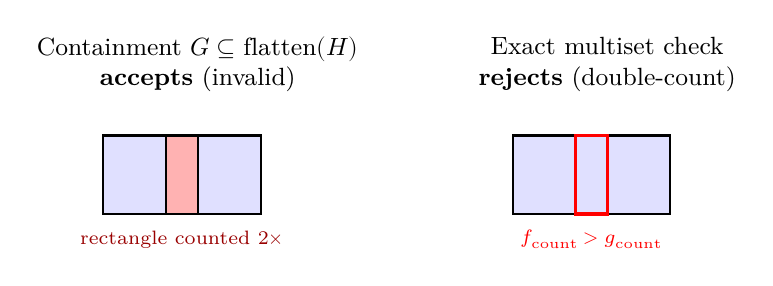
\begin{tikzpicture}[font=\footnotesize]
  \begin{scope}
    \node[align=center, font=\small] at (1.2,1.9) {Containment $G\subseteq\mathrm{flatten}(H)$\\\textbf{accepts} (invalid)};
    \fill[blue!12] (0,0) rectangle (1.2,1.0);
    \fill[blue!12] (0.8,0) rectangle (2.0,1.0);
    \fill[red!30] (0.8,0) rectangle (1.2,1.0);
    \draw[thick] (0,0) rectangle (1.2,1.0);
    \draw[thick] (0.8,0) rectangle (2.0,1.0);
    \node[font=\scriptsize, red!60!black] at (1.0,-0.32) {rectangle counted 2$\times$};
  \end{scope}
  \begin{scope}[xshift=5.2cm]
    \node[align=center, font=\small] at (1.2,1.9) {Exact multiset check\\\textbf{rejects} (double-count)};
    \fill[blue!12] (0,0) rectangle (1.2,1.0);
    \fill[blue!12] (0.8,0) rectangle (2.0,1.0);
    \draw[thick] (0,0) rectangle (1.2,1.0);
    \draw[thick] (0.8,0) rectangle (2.0,1.0);
    \draw[red, very thick] (0.8,0) rectangle (1.2,1.0);
    \node[font=\scriptsize, red] at (1.0,-0.32) {$f_{\mathrm{count}}>g_{\mathrm{count}}$};
  \end{scope}
\end{tikzpicture}
\caption{Why exact rectangle-multiset certification matters. Greedy growth over a dense periodic region can place two cell instances that overlap, reproducing a rectangle twice. A containment check ($G\subseteq\mathrm{flatten}(H)$) accepts this invalid tiling; the exact multiset check requires every real rectangle to appear with exactly its multiplicity and rejects the double-count. This is the check that caught the over-covering bug.}
\label{fig:verify}
\end{figure}

\textbf{Defect-tolerant recovery.} After clean cells are established, a
rescan accepts \textbf{partial} instances (a strong majority of members
present, \texttt{defect\_min\_support}, capped by
\texttt{defect\_max\_missing}) and records absent leaf members as a
defect layer. Under the multiset gate the constraint is that every
\emph{real} rectangle of \texttt{G} is still reproduced exactly; the
idealized-but-absent members are the defect layer
(\texttt{flatten(H)\ −\ G}, computed by Boost), so clutter overlapping a
missing member is handled (that overlap is exactly what breaks a naive
wholesale-rectangle subtraction). Missing \emph{sub-cell references} are
never tolerated, so nesting stays exact and clean tests are untouched
{[}NOTES, ``Array detection = the lattice-aligned special case''; NOTES,
``Real-GDS hierarchy-erasure''{]}.

\subsection{5.6 D4 reflection and
rotation}\label{d4-reflection-and-rotation}

For rectilinear geometry the only rigid transforms keeping rectangles
axis-aligned are the 8 elements of D4 (rotations 0/90/180/270°, each
optionally mirrored) --- exactly the GDS orientation set. The
\texttt{d4.hpp} module encodes these as signed permutation matrices with
group composition. Grouping is by a \textbf{D4-canonical signature} (the
minimum over all 8 orientations of a neighborhood's signature); matching
tries all 8; growth and flatten \textbf{compose orientations through
nesting} (a sub-cell reference's own orientation composes with its
parent's). Every instance carries an \texttt{orient} field. This is what
turns eight mirrored/rotated copies of a motif into \textbf{one} cell
definition with eight oriented instances, rather than eight unrelated
cells --- the mirrored-standard-cell-row case made to work on purpose
{[}HR, §1.2/§5.2; NOTES, Phase-2 decision 1{]}.

\subsection{5.7 The unification: array detection = one-level recovery +
lattice
fit}\label{the-unification-array-detection-one-level-recovery-lattice-fit}

The two problems are one. A cell whose recovered instances happen to lie
on a uniform 2D lattice \emph{is} an array. Concretely, run hierarchy
recovery constrained to \textbf{one level}, take the recovered cell's
instance anchors, and fit a regular axis-aligned lattice
(\texttt{fit\_lattice}) to them. The resulting
\texttt{(dx,\ dy,\ ncols,\ nrows,\ occupied,\ missing)} is precisely
what the dedicated array detector reports directly. §7.2 shows this
holds exactly on real demo data.

\begin{figure}[htb]\centering
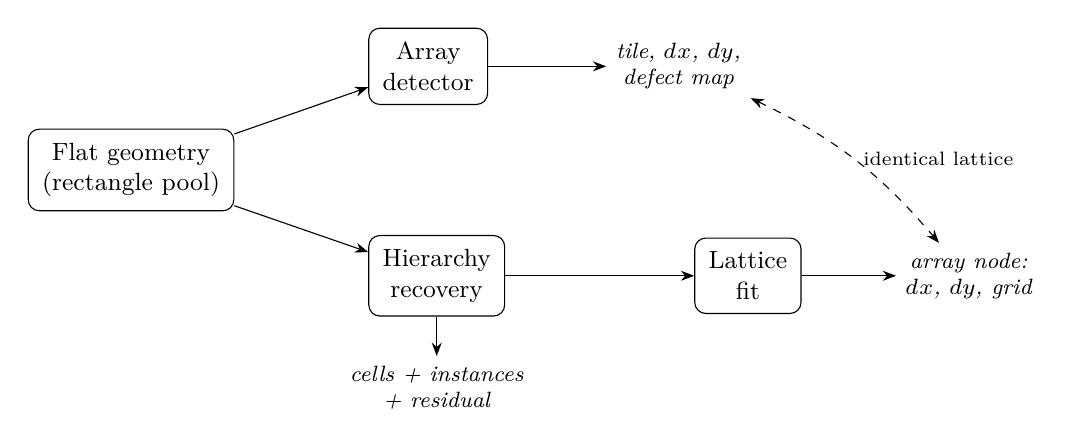
\begin{tikzpicture}[>={Stealth[]},
  b/.style={draw, rounded corners, align=center, font=\small, inner sep=5pt, minimum height=9mm},
  o/.style={align=center, font=\footnotesize\itshape}]
  \node[b] (flat) {Flat geometry\\(rectangle pool)};
  \node[b, above right=0.3cm and 1.7cm of flat] (arr) {Array\\detector};
  \node[b, below right=0.3cm and 1.7cm of flat] (hr) {Hierarchy\\recovery};
  \node[o, right=1.5cm of arr] (ao) {tile, $dx$, $dy$,\\defect map};
  \node[b, right=2.4cm of hr] (lat) {Lattice\\fit};
  \node[o, right=1.2cm of lat] (lo) {array node:\\$dx$, $dy$, grid};
  \node[o, below=0.5cm of hr] (ho) {cells + instances\\+ residual};
  \draw[->] (flat) -- (arr);  \draw[->] (flat) -- (hr);
  \draw[->] (arr) -- (ao);    \draw[->] (hr) -- (ho);
  \draw[->] (hr) -- (lat);    \draw[->] (lat) -- (lo);
  \draw[<->, dashed] (ao) to[bend left=12] node[right, font=\scriptsize] {identical lattice} (lo);
\end{tikzpicture}
\caption{The unification. Both algorithms consume the same flat geometry. The array detector yields a tile, step vectors, and a defect map directly; hierarchy recovery yields cells, instances, and residual, and a \emph{one-level} run followed by a lattice fit on the recovered instances reproduces the same lattice parameters (dashed). Array detection is the one-level, lattice-aligned special case (\S5.7, \S7.2).}
\label{fig:unify}
\end{figure}

Two honest wrinkles surface here, both informative. First,
\textbf{unconstrained} recovery need not return the array view: it can
pick a different valid decomposition (on the standard-cell layout it
returns two cells at one level rather than the single four-rectangle
array tile --- §7.2), so ``which hierarchy'' is a knob
(\texttt{max\_levels}, tie-breaks), not a fact --- the §4.4
non-uniqueness, live. Second, the correctness gate (§5.5) shapes what
unconstrained recovery \emph{can} do here: greedy MDL is tempted to keep
pairing instances into a deeper binary-doubling tree over a dense array,
but any round that would make instances overlap breaks the
exact-multiset check and is reverted, so on these dense arrays
unconstrained recovery correctly stops shallow rather than manufacturing
an invalid deeper hierarchy. Achieving \emph{valid} deep compression of
a dense lattice needs an explicit array node, not greedy doubling (§8).

\begin{center}\rule{0.5\linewidth}{0.5pt}\end{center}

\section{6. Implementation}\label{implementation}

The system is C++17 on \textbf{Boost.Geometry} (header-only, permissive
license, chosen over CGAL because the scope is rectilinear and CGAL's
exact-kernel \texttt{Arrangement\_2} machinery is more than this problem
needs). Boost provides the box/polygon primitives, the boolean set
operations for the defect computation and canonicalized equality, and
\texttt{boost::geometry::index::rtree} for the local-neighborhood
queries hierarchy recovery needs. The visualizer emits SVG directly with
no extra dependency.

Module layout (each maps to a design section):

{\def\LTcaptype{none} % do not increment counter
\begin{longtable}[]{@{}
  >{\raggedright\arraybackslash}p{(\linewidth - 2\tabcolsep) * \real{0.5000}}
  >{\raggedright\arraybackslash}p{(\linewidth - 2\tabcolsep) * \real{0.5000}}@{}}
\toprule\noalign{}
\begin{minipage}[b]{\linewidth}\raggedright
File
\end{minipage} & \begin{minipage}[b]{\linewidth}\raggedright
Stage
\end{minipage} \\
\midrule\noalign{}
\endhead
\bottomrule\noalign{}
\endlastfoot
\texttt{slab.\{hpp,cpp\}} & §5.1 scanlines: snapping + open-slab
sampling \\
\texttt{encoding.\{hpp,cpp\}} & §5.2 both encodings (occupancy merged;
edge raw/height-keyed) \\
\texttt{runs.\{hpp,cpp\}} & §5.3 per-line repetition + §5.4
defect-tolerant scan \\
\texttt{reconcile.\{hpp,cpp\}} & §5.3 compatibility predicate, CC
clustering, median/circular-median, H×V intersection \\
\texttt{verify.\{hpp,cpp\}} & §5.4 canonicalized verification +
missing/extra defect map \\
\texttt{detector.\{hpp,cpp\}} & array driver + dedup +
candidate-reduction funnel counts \\
\texttt{hierarchy.hpp} & \texttt{H} = cell defs + placements + residual
+ defect layer \\
\texttt{recover.\{hpp,cpp\}} & §5.5 shingles → grow → MDL → greedy →
recurse; \texttt{flatten(H)=G} \\
\texttt{d4.hpp} & §5.6 the 8 axis-preserving orientations \\
\texttt{bench.\{hpp,cpp\}} & §7.3 hierarchy-erasure benchmark generator
+ scorer \\
\texttt{svg\ /\ hr\_svg} & visualization \\
\end{longtable}
}

Performance-relevant implementation choices (§7.4 quantifies them):
rtree neighbor queries for shingle k-NN and growth candidates (replacing
an O(n²) per-seed distance scan); an \textbf{integer-keyed spatial hash}
(FNV over \texttt{(cell,\ orient,\ snapped-anchor)}) instead of
\texttt{std::string} keys in the hot lookup path; rtree-local,
size-capped growth; and an \textbf{O(n) exact rectangle-multiset}
verification that groups and reconstructs existing rectangles exactly
(never merging or refracturing) and compares multiplicities by hashing
snapped rectangles, instead of the iterated Boost \texttt{union\_} that
made the first correctness-focused pass O(n²).

\textbf{Verification is a correctness gate, not just a metric --- and a
linear one.} The O(n) multiset check is what makes recovery trustworthy
at scale, and it is also what \emph{caught} the over-covering bugs. An
earlier version had relaxed the check to \texttt{G\ ⊆\ flatten(H)}
(containment), which is cheap but too weak: it accepts a hierarchy in
which two nested instances overlap and reproduce a rectangle twice. That
masked a real growth bug --- in a perfectly periodic region,
seed-and-extend would add a neighbor's rectangle ``present at all
instances,'' making adjacent cell instances overlap --- and inflated the
reported compression, because the invalid, over-covering hierarchy
looked smaller than any valid one. Switching to the exact multiset check
(every real rectangle reproduced with exactly its multiplicity;
over-covering rejected as an invalid double-count; flatten-only
rectangles retained as the genuine defect layer) surfaced the bug, and
combined with the growth fix (overlap rejection + per-instance
claimed-primitive sets) and recurse-only-while-valid, it both restored
correctness and \emph{lowered} the honest compression numbers (§7.3,
§7.5). The check stays O(n): grouping and multiset comparison are
hashing passes over snapped rectangles, no Boost boolean union in the
hot path.

\begin{center}\rule{0.5\linewidth}{0.5pt}\end{center}

\section{7. Evaluation}\label{evaluation}

All numbers below are from actual runs of the implemented system,
including the §7.5 real-GDS round-trip; the only open item is the real
SKY130/ORFS crop, marked \texttt{{[}TBD{]}}.

\subsection{7.1 Correctness: bug-class regression tests and
demos}\label{correctness-bug-class-regression-tests-and-demos}

The three bug classes diagnosed in the Python prototype are reproduced
as passing regression tests (\texttt{test\_bugs}), plus the closed
encoding gap:

\begin{itemize}
\tightlist
\item
  \textbf{Bug 1 (symbol collision).} A layout where non-repeating
  clutter has, by coincidence, the exact width of a real repeated token.
  The detector still finds \texttt{dx\ =\ 20} (the true period), the 8×6
  grid, and excludes the colliding clutter from the region; all 48
  instances are clean and the clutter is not counted. Non-periodic
  content is trimmed against the canonical unit and geometric
  verification is mandatory, so a single-token width coincidence can
  neither form a period nor survive verification.
\item
  \textbf{Bug 2 (spurious sub-period from equal widths).} A repeating
  unit with an internal repeated sub-value. The detector finds
  \texttt{dx\ ≈\ 78} (the full primitive period), \emph{not} the
  \texttt{≈\ 39} half-period, because the period is chosen by
  self-consistency relative to the best achievable, not an absolute
  floor.
\item
  \textbf{Bug 3 (phase attribution across a defect).} A row/grid with a
  genuine missing instance in the middle. Of 48 expected instances,
  exactly 47 are clean and exactly one defect (type MISSING) is
  reported, \textbf{attributed to column 3, row 2 --- not shifted
  right}. The direct row-scan test confirms the mechanism: period
  \texttt{dx\ =\ 20}, 8 expected positions, one defect at physical
  \texttt{x\ =\ 60} (start of instance 3), not shifted. The defect scan
  walks expected physical positions, never token indices.
\item
  \textbf{Zero-gap gap closure.} A directly-abutted standard-cell array
  (which occupancy alone cannot see) is detected via the edge encoding.
\end{itemize}

Array-detection demos (\texttt{demo}), with the candidate-reduction
funnel \texttt{N} symbolic runs ≫ \texttt{M} clusters ≫ \texttt{K}
verified arrays:

{\def\LTcaptype{none} % do not increment counter
\begin{longtable}[]{@{}
  >{\raggedright\arraybackslash}p{(\linewidth - 16\tabcolsep) * \real{0.1111}}
  >{\raggedright\arraybackslash}p{(\linewidth - 16\tabcolsep) * \real{0.1111}}
  >{\raggedright\arraybackslash}p{(\linewidth - 16\tabcolsep) * \real{0.1111}}
  >{\raggedright\arraybackslash}p{(\linewidth - 16\tabcolsep) * \real{0.1111}}
  >{\raggedright\arraybackslash}p{(\linewidth - 16\tabcolsep) * \real{0.1111}}
  >{\raggedright\arraybackslash}p{(\linewidth - 16\tabcolsep) * \real{0.1111}}
  >{\raggedright\arraybackslash}p{(\linewidth - 16\tabcolsep) * \real{0.1111}}
  >{\raggedright\arraybackslash}p{(\linewidth - 16\tabcolsep) * \real{0.1111}}
  >{\raggedright\arraybackslash}p{(\linewidth - 16\tabcolsep) * \real{0.1111}}@{}}
\toprule\noalign{}
\begin{minipage}[b]{\linewidth}\raggedright
Demo
\end{minipage} & \begin{minipage}[b]{\linewidth}\raggedright
Rects
\end{minipage} & \begin{minipage}[b]{\linewidth}\raggedright
Runs N
\end{minipage} & \begin{minipage}[b]{\linewidth}\raggedright
Clusters M
\end{minipage} & \begin{minipage}[b]{\linewidth}\raggedright
Verified K
\end{minipage} & \begin{minipage}[b]{\linewidth}\raggedright
dx
\end{minipage} & \begin{minipage}[b]{\linewidth}\raggedright
dy
\end{minipage} & \begin{minipage}[b]{\linewidth}\raggedright
Grid
\end{minipage} & \begin{minipage}[b]{\linewidth}\raggedright
Clean / Missing / Extra
\end{minipage} \\
\midrule\noalign{}
\endhead
\bottomrule\noalign{}
\endlastfoot
bauhaus (decorative) & 101 & 58 & 2 & 1 & 40 & 40 & 8×6 & 47 / 1 / 0 \\
standard-cell (gapped rows) & 109 & 109 & 5 & 1 & 87 & 26 & 5×5 & 24 / 1
/ 15 \\
standard-cell (zero-gap abutted) & 102 & 45 & 2 & 1 & 79 & 26 & 5×5 & 24
/ 1 / 0 \\
\end{longtable}
}

The gapped standard-cell demo carries 15 routing overlays
(\texttt{extra}) and one genuine missing cell (\texttt{missing}, area
356.4), reported distinctly --- the value of the defect model. The
abutted demo isolates the encoding point: edge encoding recovers
zero-gap geometry occupancy cannot. (Per NOTES, the abutted demo
deliberately uses non-crossing border clutter, because edge-only
encoding is clutter-fragile over zero-gap geometry --- see §8.)

\begin{figure}
\centering
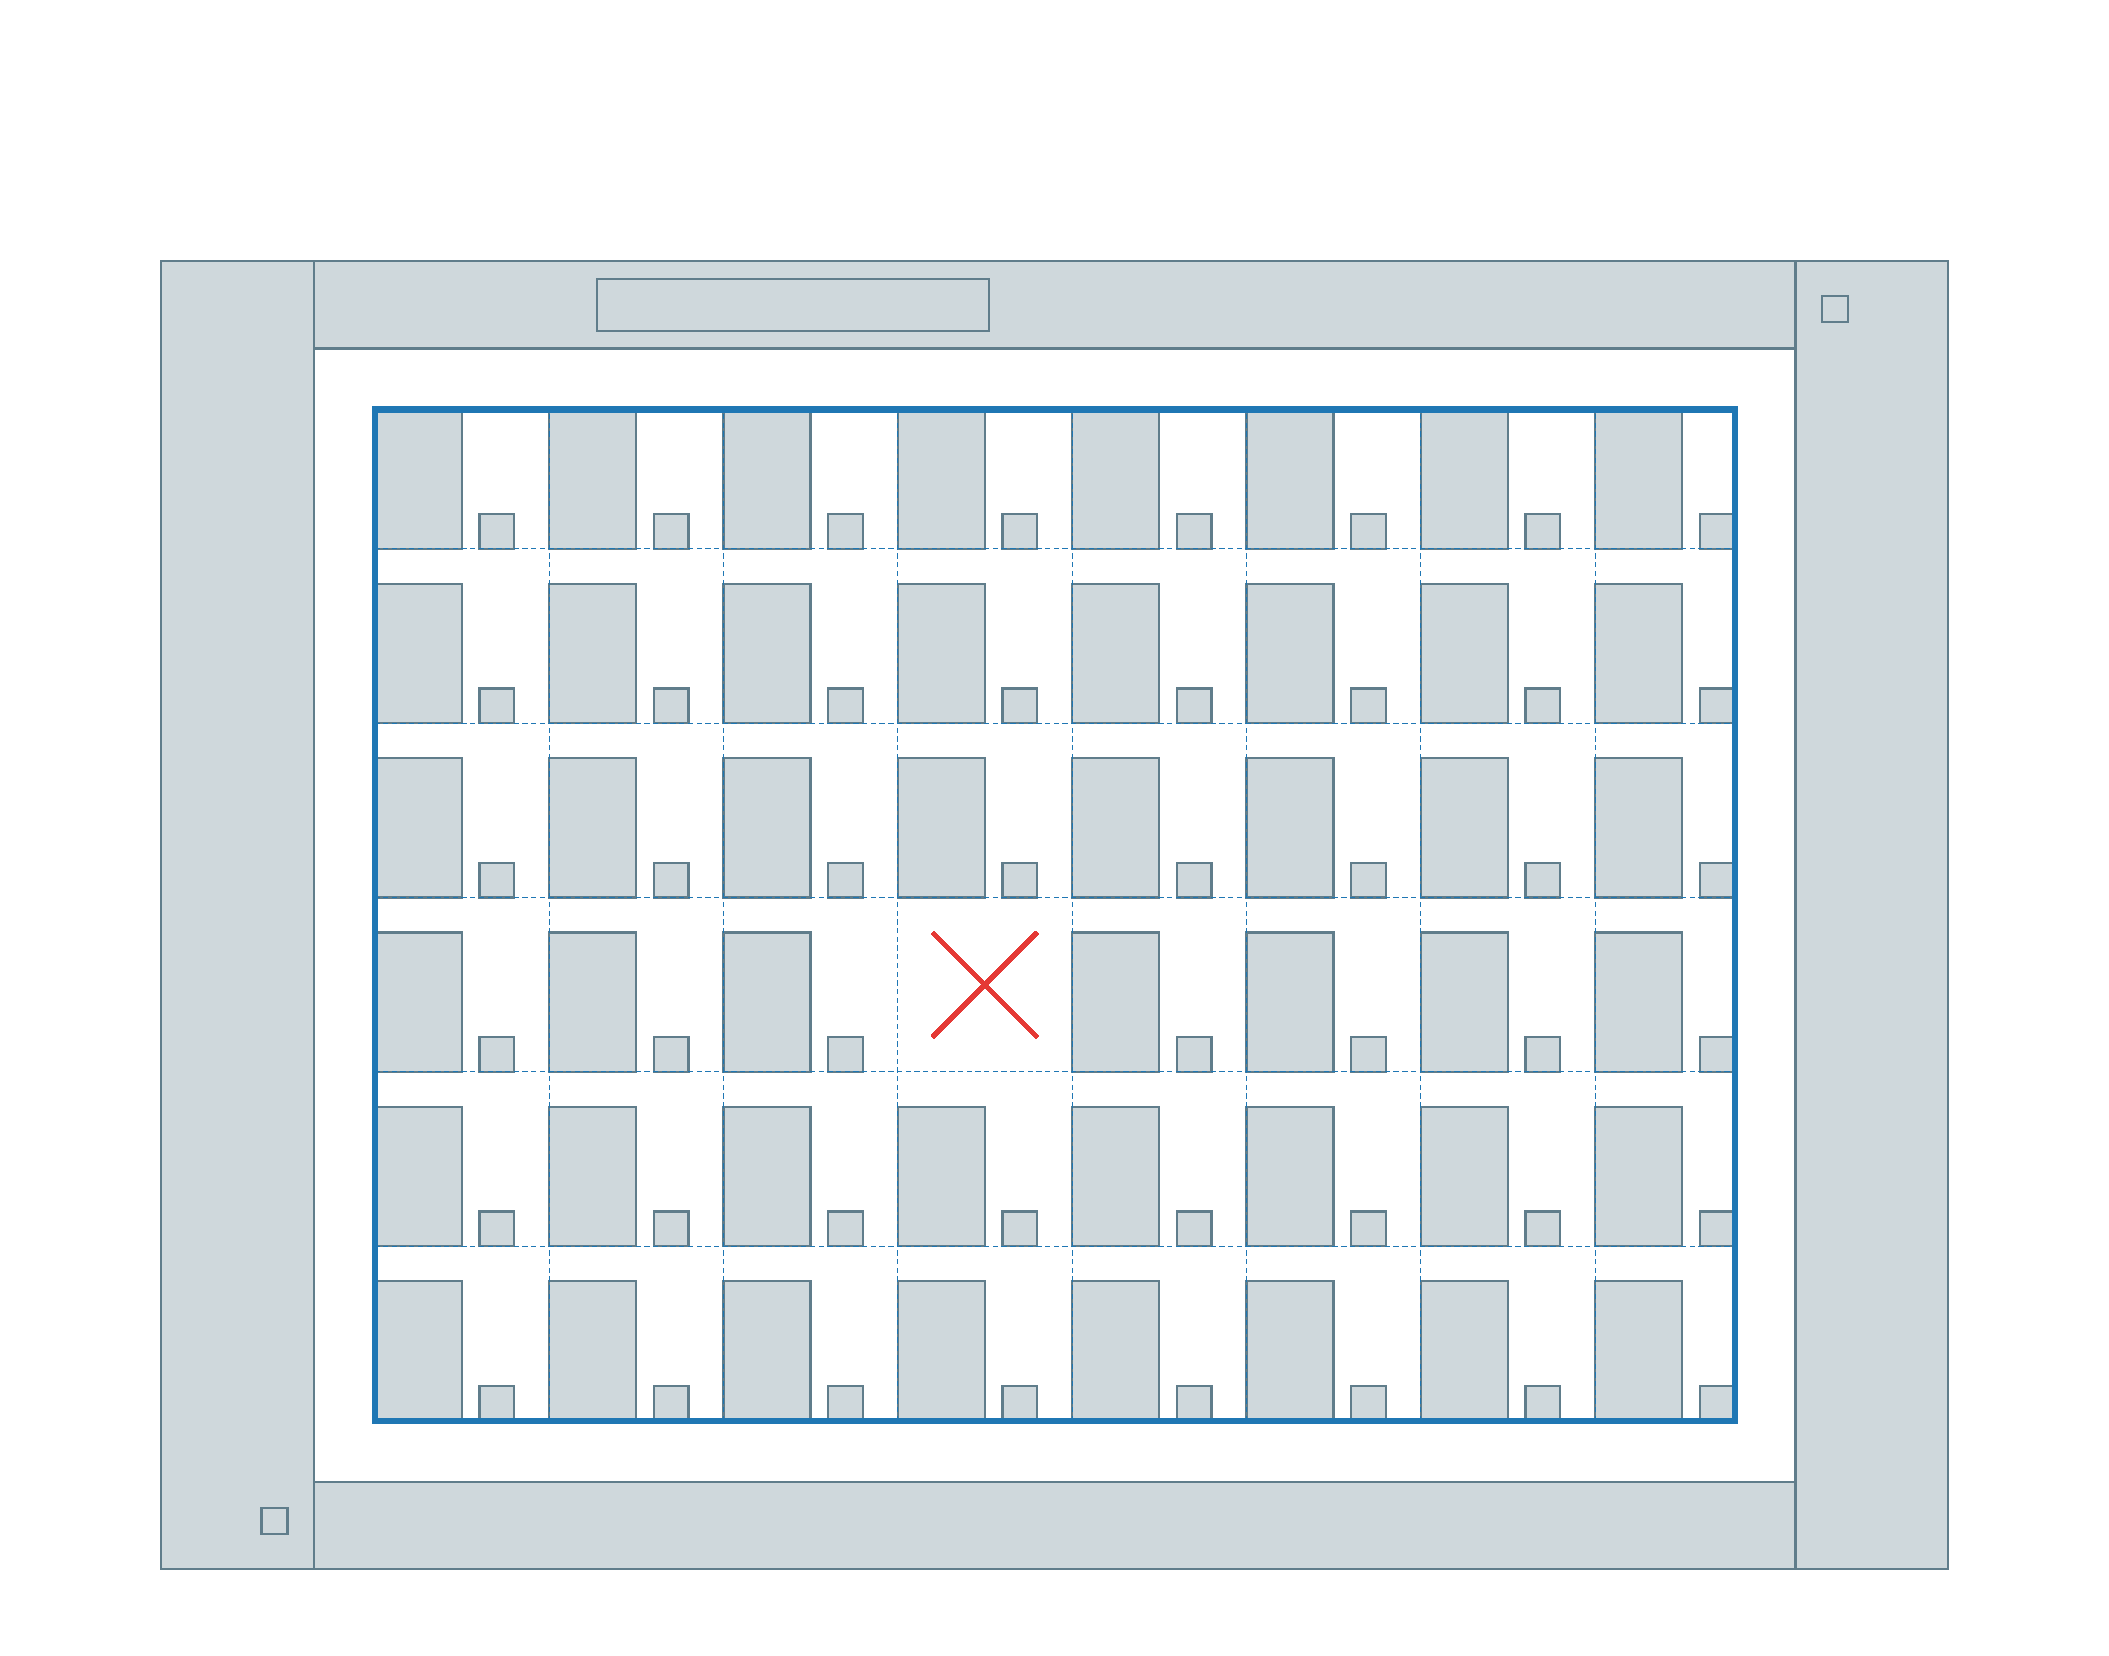
\includegraphics[width=0.68\linewidth,height=\textheight,keepaspectratio,alt={Array detection on the decorative bauhaus demo. The detected 8×6 array region (blue outline) excludes the non-repeating decorative border, title bar, and corner ornaments; the dashed lattice shows the recovered dx = dy = 40 step; the red × marks the single deliberately-missing motif. Result: 47 clean instances, 1 defect, exact.}]{figures/bauhaus.pdf}
\caption{Array detection on the decorative \emph{bauhaus} demo. The
detected 8×6 array region (blue outline) excludes the non-repeating
decorative border, title bar, and corner ornaments; the dashed lattice
shows the recovered \(dx = dy = 40\) step; the red × marks the single
deliberately-missing motif. Result: 47 clean instances, 1 defect,
exact.}
\end{figure}

Hierarchy-recovery demos (\texttt{hr\_demo}):

{\def\LTcaptype{none} % do not increment counter
\begin{longtable}[]{@{}
  >{\raggedright\arraybackslash}p{(\linewidth - 8\tabcolsep) * \real{0.2000}}
  >{\raggedright\arraybackslash}p{(\linewidth - 8\tabcolsep) * \real{0.2000}}
  >{\raggedright\arraybackslash}p{(\linewidth - 8\tabcolsep) * \real{0.2000}}
  >{\raggedright\arraybackslash}p{(\linewidth - 8\tabcolsep) * \real{0.2000}}
  >{\raggedright\arraybackslash}p{(\linewidth - 8\tabcolsep) * \real{0.2000}}@{}}
\toprule\noalign{}
\begin{minipage}[b]{\linewidth}\raggedright
Demo
\end{minipage} & \begin{minipage}[b]{\linewidth}\raggedright
Leaf rects
\end{minipage} & \begin{minipage}[b]{\linewidth}\raggedright
Cells
\end{minipage} & \begin{minipage}[b]{\linewidth}\raggedright
Levels
\end{minipage} & \begin{minipage}[b]{\linewidth}\raggedright
Result
\end{minipage} \\
\midrule\noalign{}
\endhead
\bottomrule\noalign{}
\endlastfoot
nested motif (irregular placement) & 29 & 2 & 2 & leaf cell ×13,
super-cell (3 refs to leaf) ×3, 7 top, 3 residual; 1.93× \\
oriented motif (all 8 D4) & 18 & 1 & 1 & one cell, 8 instances spanning
o0..o7; 1.50× \\
defective motif & 20 & 1 & 1 & one 4-member cell ×5, one instance
missing a member; defect area 120 \\
\end{longtable}
}

All three satisfy \texttt{G\ ⊆\ flatten(H)}. The oriented case is the D4
payoff: eight mirrored/rotated copies collapse to one cell. The
defective case exercises defect-tolerant recovery end to end.

\subsection{7.2 The unification result}\label{the-unification-result}

On identical flat input, the dedicated array detector and one-level
hierarchy recovery + lattice fit (\texttt{unify\_demo},
\texttt{test\_unify}) produce identical lattices:

{\def\LTcaptype{none} % do not increment counter
\begin{longtable}[]{@{}
  >{\raggedright\arraybackslash}p{(\linewidth - 14\tabcolsep) * \real{0.1250}}
  >{\raggedright\arraybackslash}p{(\linewidth - 14\tabcolsep) * \real{0.1250}}
  >{\raggedright\arraybackslash}p{(\linewidth - 14\tabcolsep) * \real{0.1250}}
  >{\raggedright\arraybackslash}p{(\linewidth - 14\tabcolsep) * \real{0.1250}}
  >{\raggedright\arraybackslash}p{(\linewidth - 14\tabcolsep) * \real{0.1250}}
  >{\raggedright\arraybackslash}p{(\linewidth - 14\tabcolsep) * \real{0.1250}}
  >{\raggedright\arraybackslash}p{(\linewidth - 14\tabcolsep) * \real{0.1250}}
  >{\raggedright\arraybackslash}p{(\linewidth - 14\tabcolsep) * \real{0.1250}}@{}}
\toprule\noalign{}
\begin{minipage}[b]{\linewidth}\raggedright
Layout
\end{minipage} & \begin{minipage}[b]{\linewidth}\raggedright
Path
\end{minipage} & \begin{minipage}[b]{\linewidth}\raggedright
dx
\end{minipage} & \begin{minipage}[b]{\linewidth}\raggedright
dy
\end{minipage} & \begin{minipage}[b]{\linewidth}\raggedright
Grid
\end{minipage} & \begin{minipage}[b]{\linewidth}\raggedright
Occupied
\end{minipage} & \begin{minipage}[b]{\linewidth}\raggedright
Missing
\end{minipage} & \begin{minipage}[b]{\linewidth}\raggedright
flatten=G
\end{minipage} \\
\midrule\noalign{}
\endhead
\bottomrule\noalign{}
\endlastfoot
bauhaus (101 rects) & array detector & 40 & 40 & 8×6 & 47 & 1 & --- \\
bauhaus & 1-level recovery + lattice fit & 40 & 40 & 8×6 & 47 & 1 &
yes \\
standard-cell (109 rects) & array detector & 87 & 26 & 5×5 & 24 & 1 &
--- \\
standard-cell & 1-level recovery + lattice fit & 87 & 26 & 5×5 & 23 & 2
& yes \\
\end{longtable}
}

\texttt{test\_unify} asserts these match: array
\texttt{dx}/\texttt{dy}/grid equal the lattice-fit values, and occupied
+ missing equals the array instance count. (On standard-cell the two
paths partition the same sites slightly differently between ``occupied''
and ``missing'' --- 23+2 vs 24+1 --- because one-level recovery groups
by exact modal-cell membership while the array verifier's modal-tile
clip counts one borderline instance as clean; both agree on the lattice
and both satisfy their correctness constraint.) The unconstrained
full-hierarchy path finds a \emph{different} valid decomposition on each
layout --- bauhaus: 1 cell at 1 level, cost 56 vs.~flat 101 (1.80×);
standard-cell: 2 cells at 1 level, cost 43 vs.~109 (2.53×) --- a live
instance of §4.4 non-uniqueness. (Under the corrected exact-multiset
gate, unconstrained recovery on these dense arrays now stays shallow
rather than manufacturing the deeper binary-doubling tree an earlier
over-covering path reported; see §5.5, §5.7.) \textbf{This equality
between the two independent paths is the paper's core empirical claim:
array detection is the one-level lattice-aligned special case of
hierarchy recovery, demonstrated, not asserted.}

\subsection{7.3 Hierarchy-erasure
benchmark}\label{hierarchy-erasure-benchmark}

The benchmark (\texttt{bench}, \texttt{erasure\_demo}) builds a design
with \textbf{known} hierarchy --- a leaf 4-rectangle ``gate'' → a
horizontal array ``slice'' → a vertical stack of alternately-mirrored
slices ``block'' → a row of blocks ``chip'' --- flattens it to raw
rectangles, strips all cell/instance/array metadata, and asks the
recoverer to reconstruct a compact hierarchy from geometry alone. Ground
truth is the design's own construction, so nothing is hand-labeled.
Compression is \texttt{flat\ leaf\ count\ /\ hierarchy\ cost}.

{\def\LTcaptype{none} % do not increment counter
\begin{longtable}[]{@{}
  >{\raggedright\arraybackslash}p{(\linewidth - 18\tabcolsep) * \real{0.1000}}
  >{\raggedright\arraybackslash}p{(\linewidth - 18\tabcolsep) * \real{0.1000}}
  >{\raggedright\arraybackslash}p{(\linewidth - 18\tabcolsep) * \real{0.1000}}
  >{\raggedright\arraybackslash}p{(\linewidth - 18\tabcolsep) * \real{0.1000}}
  >{\raggedright\arraybackslash}p{(\linewidth - 18\tabcolsep) * \real{0.1000}}
  >{\raggedright\arraybackslash}p{(\linewidth - 18\tabcolsep) * \real{0.1000}}
  >{\raggedright\arraybackslash}p{(\linewidth - 18\tabcolsep) * \real{0.1000}}
  >{\raggedright\arraybackslash}p{(\linewidth - 18\tabcolsep) * \real{0.1000}}
  >{\raggedright\arraybackslash}p{(\linewidth - 18\tabcolsep) * \real{0.1000}}
  >{\raggedright\arraybackslash}p{(\linewidth - 18\tabcolsep) * \real{0.1000}}@{}}
\toprule\noalign{}
\begin{minipage}[b]{\linewidth}\raggedright
Case
\end{minipage} & \begin{minipage}[b]{\linewidth}\raggedright
Rects
\end{minipage} & \begin{minipage}[b]{\linewidth}\raggedright
Cells
\end{minipage} & \begin{minipage}[b]{\linewidth}\raggedright
Levels
\end{minipage} & \begin{minipage}[b]{\linewidth}\raggedright
Top insts
\end{minipage} & \begin{minipage}[b]{\linewidth}\raggedright
Residual
\end{minipage} & \begin{minipage}[b]{\linewidth}\raggedright
Defective
\end{minipage} & \begin{minipage}[b]{\linewidth}\raggedright
Compression
\end{minipage} & \begin{minipage}[b]{\linewidth}\raggedright
flatten=G (exact)
\end{minipage} & \begin{minipage}[b]{\linewidth}\raggedright
Leaf found
\end{minipage} \\
\midrule\noalign{}
\endhead
\bottomrule\noalign{}
\endlastfoot
flat array (1 block) & 96 & 1 & 1 & 24 & 0 & 0 & \textbf{3.43×} & YES &
found \\
nested ×2 blocks & 196 & 1 & 1 & 47 & 8 & 0 & \textbf{3.32×} & YES &
found \\
nested + mirrored rows & 246 & 1 & 1 & 59 & 10 & 0 & \textbf{3.37×} &
YES & found \\
larger + mirrored + clutter & 588 & 1 & 1 & 142 & 20 & 0 &
\textbf{3.54×} & YES & found \\
\end{longtable}
}

Every case satisfies the exact rectangle-multiset flatten check (not
merely containment) and recovers the ground-truth leaf gate; compression
is \textbf{\textasciitilde3.3--3.5×}. The mirrored cases exercise D4
(adjacent rows share a rail). These numbers replace an earlier, higher
figure (\textasciitilde5--8×) that came from the over-covering
verification bug described in §6: under the weak \texttt{G\ ⊆\ flatten}
check, invalid hierarchies whose nested instances overlapped were
accepted and looked artificially smaller. The corrected exact-multiset
gate both rejects those and reports the honest, valid compression. Note
also that the recovered hierarchies now stay at \textbf{one level} on
these dense arrays: recurse-only-while-valid reverts any deeper round
that would break exactness, so greedy binary doubling cannot fragment
the lattice into an invalid tree. The consequence is that \emph{valid
deep compression of a dense array is left on the table} --- capturing it
needs an explicit array node (represent a K-instance lattice as one
array node rather than a log-K doubling tree), which is future work
(§8). Defect tolerance is also demonstrated in recovery: on a defective
datapath the missing gate member is recorded as the defect layer while
every real rectangle is still reproduced exactly.

\subsection{7.4 Performance and
scalability}\label{performance-and-scalability}

The recovery pipeline was profiled after a first correctness-focused
pass revealed an O(n²) blowup (a \textasciitilde1000-rectangle design
took minutes). Phase-by-phase timing showed \textbf{the algorithm was
never the bottleneck}: the per-round work (shingle / group / build /
dedup / greedy) was already linear and fast --- about \textbf{6 ms at n
= 3072}. The entire O(n²) lived in the final \texttt{flatten(H)\ =\ G}
verification, which built one giant multipolygon by iterated Boost
\texttt{union\_}.

The four fixes (rtree neighbor queries, integer-keyed spatial hash,
rtree-local size-capped growth, and the O(n) exact rectangle-multiset
verification --- §6) removed the quadratic term entirely. The resulting
scaling:

{\def\LTcaptype{none} % do not increment counter
\begin{longtable}[]{@{}
  >{\raggedright\arraybackslash}p{(\linewidth - 2\tabcolsep) * \real{0.5000}}
  >{\raggedright\arraybackslash}p{(\linewidth - 2\tabcolsep) * \real{0.5000}}@{}}
\toprule\noalign{}
\begin{minipage}[b]{\linewidth}\raggedright
Metric
\end{minipage} & \begin{minipage}[b]{\linewidth}\raggedright
Value
\end{minipage} \\
\midrule\noalign{}
\endhead
\bottomrule\noalign{}
\endlastfoot
Per-rectangle cost & \textasciitilde3 µs/rect, linear \\
Per-round work at n = 3072 & \textasciitilde6 ms \\
1.58 M rectangles, single round & \textasciitilde4.8 s (one core) \\
1.58 M rectangles, full 8-level recursion & \textasciitilde30 s (one
core) \\
Correctness (exact rectangle-multiset flatten check) & intact at all
sizes \\
\end{longtable}
}

The key methodological finding: \textbf{the interesting bottleneck was
verification, not detection.} Once verification is made linear, the
whole pipeline is linear --- and, as §6 recounts, making that
verification \emph{exact} (rather than a cheaper containment test) is
also what caught the over-covering bug, so the correctness gate and the
performance fix are the same piece of code.

Path to billions (architecture ready, not yet built): \textbf{tiling +
parallelism} (rounds, tiles, and candidates are independent; the rtree
and per-tile recovery parallelize cleanly, with a stitch pass for motifs
crossing tile borders); \textbf{streaming / out-of-core} for layouts
exceeding RAM; \textbf{array-node compression} (represent a large
lattice as one O(1) array node, which also captures the valid deep
compression §7.3 currently leaves on the table); and applying the same
O(n) rectangle approach to the array detector's own verifier, which
still uses the iterated-union pattern.

\subsection{7.5 Real-GDS
hierarchy-erasure}\label{real-gds-hierarchy-erasure}

The real-GDS round-trip benchmark exercises genuine GDS I/O and real
flattening (the geometry is synthetic; a real open-source GDS crop is
the remaining step, below). \texttt{scripts/gds\_roundtrip.py} uses
\texttt{gdstk} to \textbf{write} a genuinely hierarchical \texttt{.gds}:
a leaf \texttt{gate} cell (4 rectangles), a \texttt{slice} built as an
array reference (AREF) of the gate, a \texttt{block} of alternately
\texttt{x\_reflection}-mirrored slices (the way place-and-route mirrors
standard-cell rows to share a power rail), a \texttt{top} of blocks,
plus routing clutter. It then \textbf{reads the file back and flattens
it with the tool}, discarding all cell/instance/array metadata, and
exports the flat rectangles. \texttt{build/gds\_recover} recovers a
hierarchy from those flat rectangles alone. The geometry is synthetic,
but the GDS format, the hierarchy, the mirroring, and the flatten are
all real --- and dropping in a real \textbf{SKY130}/ORFS \texttt{.gds}
uses the identical read → flatten → export path.

Measured result:

{\def\LTcaptype{none} % do not increment counter
\begin{longtable}[]{@{}
  >{\raggedright\arraybackslash}p{(\linewidth - 2\tabcolsep) * \real{0.5000}}
  >{\raggedright\arraybackslash}p{(\linewidth - 2\tabcolsep) * \real{0.5000}}@{}}
\toprule\noalign{}
\begin{minipage}[b]{\linewidth}\raggedright
Quantity
\end{minipage} & \begin{minipage}[b]{\linewidth}\raggedright
Value
\end{minipage} \\
\midrule\noalign{}
\endhead
\bottomrule\noalign{}
\endlastfoot
Flattened rectangles (G) & 772 \\
Ground truth & 4 designer cells (gate/slice/block/top), 4 levels, gate =
4 rects × \textbf{192} instances \\
Recovered & \textbf{1 cell of 4 rectangles}, 1 level, \textbf{191} top
placements, 8 residual rectangles \\
Leaf gate recovered & YES (4-rectangle cell) \\
flatten(H) = G & \textbf{YES, exact} (rectangle-multiset check) \\
Compression & \textbf{3.80×} (flat 772 → hierarchy 203) \\
\end{longtable}
}

\begin{figure}
\centering
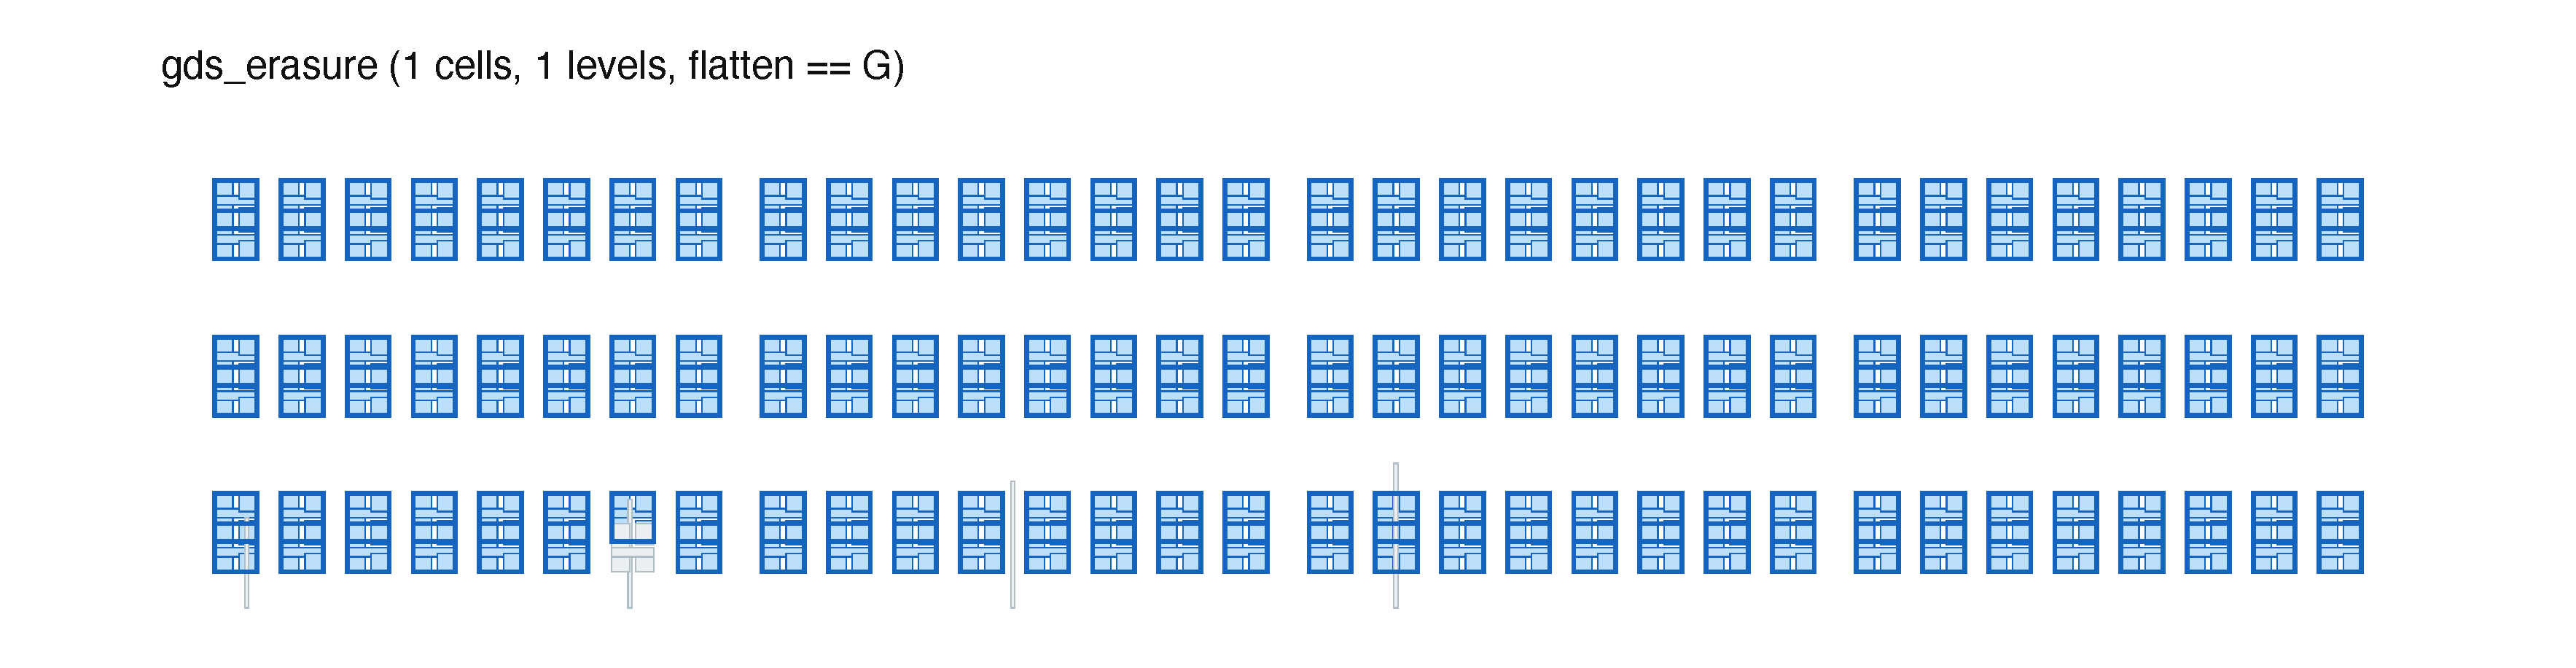
\includegraphics[width=0.92\linewidth,height=\textheight,keepaspectratio,alt={Recovery from a flattened, metadata-stripped real GDS. The hierarchical .gds (gate → slice → block → top, with mirrored rows) is written and flattened by gdstk; the recoverer reconstructs the 4-rectangle gate cell as instances across the layout (blue), with routing clutter left as residual (gray), flatten(H) = G exact.}]{figures/hierarchy_gds.pdf}
\caption{Recovery from a flattened, metadata-stripped real GDS. The
hierarchical \protect\texttt{.gds} (gate → slice → block → top, with
mirrored rows) is written and flattened by \protect\texttt{gdstk}; the
recoverer reconstructs the 4-rectangle gate cell as instances across the
layout (blue), with routing clutter left as residual (gray),
\protect\texttt{flatten(H)\ =\ G} exact.}
\end{figure}

The recoverer reconstructs the ground-truth 4-rectangle gate cell at
\textbf{191 of 192} instances; one edge gate falls to residual, and the
clutter is left as residual --- exactly the kind of principled
disagreement §4.4 predicts. We therefore report this as
\textbf{agreement, not accuracy} {[}HR, §1.3{]}: the recovered hierarchy
is a compact, geometrically exact decomposition
(\texttt{flatten(H)\ =\ G} holds exactly under the multiset gate), which
need not match the designer's four-level gate/slice/block/top
decomposition. The 3.80× compression sits at the top of the corrected
\textasciitilde3.3--3.8× range and, like the synthetic cases, is
one-level --- the deeper valid compression of the dense mirrored array
again awaits array-node support (§8).

This is also the evaluation that surfaced the over-covering verification
bug (§6): the dense, mirrored, abutting arrays in a real flattened GDS
are precisely the stress case that made adjacent-instance overlap
possible, which the exact-multiset gate then rejected.

The remaining source per the design's three-source scoping
recommendation {[}v4, §7.3{]} --- a real flattened crop from the
\textbf{SkyWater SKY130} PDK / \textbf{OpenROAD-flow-scripts (ORFS)}
flow --- plugs into the same path; \texttt{FreePDK45}/Nangate-style
libraries are a classic academic baseline and \texttt{ALIGN} analog
layouts (matched-device / capacitor arrays) a harder stretch target.
\textbf{{[}TBD{]}} run the identical harness on a real SKY130/ORFS
\texttt{.gds} crop and report the same metrics row.

\begin{center}\rule{0.5\linewidth}{0.5pt}\end{center}

\section{8. Limitations and
Non-Uniqueness}\label{limitations-and-non-uniqueness}

We follow the design documents in being explicit about what the
framework does \emph{not} claim.

\textbf{Recovered hierarchy is one of many valid decompositions.} This
is the central honesty point {[}HR, §1.3, §2.8{]}. A flat layout admits
many geometrically valid hierarchies; both the greedy selection
(order-dependent) and the recursion (operating on whatever partial
compression the previous level produced) mean the output is one member
of a family, not a canonical answer. We saw it live in §7.2
(unconstrained recovery picks a different decomposition from the array
view) and in §7.5 (191 of 192 gates recovered, the 192nd falling to
residual --- a principled disagreement, not an error). Where a source
hierarchy is known, we therefore report \textbf{agreement, not accuracy}
--- a well-formed inferred hierarchy can legitimately disagree with a
designer's decomposition while flattening to identical geometry. The
knobs (\texttt{max\_levels}, \texttt{min\_cell\_members},
\texttt{cost\_instance}, \texttt{gain\_min}, \ldots) are the controls
that select \emph{which} valid hierarchy is returned; they are
non-uniqueness controls, not accuracy dials.

\textbf{Greedy selection is non-optimal.} Selection is weighted
set-packing (NP-hard in general); the greedy heuristic has no optimality
guarantee. ILP for small/medium candidate counts, and a principled
global objective, are explicit future work {[}HR, §2.7{]}.

\textbf{Edge-only encoding is clutter-fragile.} Occupancy leans on gap
structure to stay robust to routing wires crossing an array (the gapped
standard-cell demo has crossing wires and detects perfectly). The edge
encoding has no gaps to anchor on, so clutter crossing \textbf{zero-gap}
geometry perturbs the token stream and can push individual rows to
spurious periods. The abutted demo therefore uses non-crossing border
clutter, isolating the point it exists to make (edge encoding recovers
directly-abutted geometry occupancy cannot) without implying an
edge-encoding clutter-robustness the design does not yet claim. An
occupancy-vs-edge ablation over routed real layouts is open {[}NOTES,
``One honest limitation''; v4, §9 Q9{]}.

\textbf{Fractured-polygon verification not yet implemented.} Recovery's
exact rectangle-multiset match certifies one logical shape only when its
rectangles match without edge-merging. A shape fractured differently
between two instances would need the array verifier's canonicalization
(merge coincident edges before comparison) reused in the recovery path
--- flagged, not built {[}NOTES, Phase-2 decision 6{]}.

\textbf{Valid deep compression of dense arrays is left on the table.}
Greedy MDL is tempted to compress a dense lattice with a deep
binary-doubling tree, but on a contiguous array such doubling makes
nested instances overlap, which the exact-multiset gate (§6) correctly
rejects --- so recovery reverts those rounds and stops at one level.
This is the honest post-fix behavior: every benchmark case (§7.3) and
the real GDS (§7.5) recovers the leaf and flattens exactly, but at a
modest \textasciitilde3.3--3.8× rather than the deeper compression a
dense array could in principle admit. (An earlier, higher figure of
\textasciitilde5--8× was the \emph{invalid} over-covering path that the
weak containment check accepted; it is not a target to recover.)
Capturing valid deep compression needs \textbf{array-node compression}
--- represent a K-instance lattice as one explicit array node
(\texttt{(tile,\ dx,\ dy,\ count)}) rather than a placement list or a
log-K doubling tree --- which is also on the scalability path (§7.4).
This is exactly where the framework closes back on itself: an array node
\emph{is} the array detector's output, so array-node compression is the
natural mechanism for a recovered cell whose instances happen to lie on
a lattice. Future work.

\textbf{Other scoped-out items.} Multi-layer / multi-class geometry,
holes and overlapping polygons, oblique (non-orthogonal) lattices, and
the §4 candidate-scoring formula (normalized-product
vs.~log-weighted-sum, left unimplemented because verification alone
suffices at demo scale {[}NOTES, decision 8{]}) are all out of the
current scope.

\begin{center}\rule{0.5\linewidth}{0.5pt}\end{center}

\section{9. Conclusion and Future
Work}\label{conclusion-and-future-work}

We have presented a single geometry-first framework for recovering
repeated structure in flat 2D rectilinear layouts, spanning rigid
lattice arrays through arbitrary nested hierarchy, unified by two shared
mechanisms: canonicalized geometric equality as the only certifier
(symbolic string and local-hash methods are candidate generators, never
proofs), and an MDL compression-gain objective as the promotion rule.
The unification is not rhetorical --- array detection is realized as
one-level hierarchy recovery plus a lattice fit, and the two independent
paths produce identical lattice parameters (step vectors and grid) with
equivalent total site accounting on real demo data, differing only in
one modal-cell attribution on the standard-cell case (§7.2). The system
reproduces three previously-diagnosed bug classes as passing regression
tests, handles zero-gap abutted geometry through a second encoding,
recovers D4-oriented instances as one cell, and passes both a synthetic
and a real-GDS hierarchy-erasure benchmark with exact rectangle-multiset
flatten-equality and \textasciitilde3.3--3.8× compression, recovering
the leaf cell in every case, running linearly at \textasciitilde3
µs/rect (1.58 M rectangles in \textasciitilde4.8 s single-round on one
core). A methodological point worth carrying forward: the exact
verification is a correctness gate, not a scoreboard --- it caught an
over-covering bug that a cheaper containment check had hidden, and
lowering the reported compression to the honest range was the
\emph{right} outcome, not a regression. The framework is honest about
non-uniqueness throughout: agreement, not accuracy.

\textbf{Future work}, in rough priority order: (1) run the identical
\texttt{gdstk} harness on a real SKY130/ORFS \texttt{.gds} crop (§7.5);
(2) \textbf{array-node compression} to represent dense lattices as O(1)
array nodes --- capturing the valid deep compression currently left on
the table and closing the framework on itself, since an array node is
exactly the array detector's output; (3) \textbf{tiling + parallelism}
and streaming toward billion-polygon layouts; (4)
\textbf{fractured-polygon verification} in the recovery path via reused
canonicalization; (5) the \textbf{Channel A} multi-serialization
generator and an occupancy-vs-edge and Channel-A-vs-B \textbf{ablation};
(6) ILP/global selection to replace greedy; and (7) multi-layer support.
Papers on either algorithm should follow real, benchmarked output ---
this draft is the working record toward that, not a finished result.

\begin{center}\rule{0.5\linewidth}{0.5pt}\end{center}

\section{References}\label{references}

\begin{itemize}
\tightlist
\item
  \textbf{{[}v4{]}} \emph{Geometry-First Array Detection in 2D Polygon
  Layouts via 1D Repetition Hypotheses}, v4
  (\texttt{repeat-cell-detection-proposal-v4.md}). The array-detection
  design of record.
\item
  \textbf{{[}HR{]}} \emph{Hierarchy Recovery from Flattened Polygon
  Layouts via Repetition-Driven Compression}, v1
  (\texttt{hierarchy-recovery-proposal-v1.md}). The companion
  hierarchy-recovery design.
\item
  \textbf{{[}NOTES{]}} \emph{Phase 1 --- implementation notes \& flagged
  design decisions} (\texttt{NOTES.md}). Design decisions taken where
  the proposals left choices open, measured performance, and honest
  limitations.
\item
  SkyWater \textbf{SKY130} PDK:
  https://skywater-pdk.readthedocs.io/en/main/contents.html
\item
  \textbf{OpenROAD-flow-scripts (ORFS)}:
  https://openroad-flow-scripts.readthedocs.io/en/latest/
\item
  OpenROAD Project (background):
  https://en.wikipedia.org/wiki/OpenROAD\_Project
\item
  \textbf{ALIGN} (analog layout automation):
  https://align-analoglayout.github.io/ALIGN-public/
\item
  \textbf{FreePDK45 / Nangate}-style open standard-cell libraries
  (classic academic baseline).
\item
  \textbf{DeepPCB} (secondary raster baseline only):
  https://github.com/tangsanli5201/DeepPCB
\end{itemize}

\end{document}
